% Agent-derived proof and independent checks:
% topics/products/pentagon-arbitrary-partner/symmetric-partner-lemma.md
% Reader-facing rewrite: symmetric-partner-exposition.md in that topic.
% Inclusion selected by Joern: docs/project-facts.md, item 13.2.
\section{A regular pentagon with a centrally symmetric partner}
\label{sec:pentagon-symmetric-partner}

The preceding section allowed the two pentagons to deform independently.
We now keep one regular pentagon fixed and allow its partner to be any
centrally symmetric planar convex body, including a smooth body.
Capacity becomes the largest scale of one prescribed regular decagon that
fits inside the partner. The same decagon uniquely maximizes the systolic
ratio in this class.\footnote{The reference-cover argument in this section
was developed and independently checked by Codex agents. This records agent
review, not completed personal verification or publication novelty.}

Keep the preceding normal convention, and put
\[
 \theta=\frac\pi5,\qquad h=\cos\theta,\qquad
 n_i=(\cos(2\pi i/5),\sin(2\pi i/5)),\qquad
 Q=\{p:n_i\cdot p\le h,\ 0\le i<5\}.
\]
Thus $Q$ has circumradius one. Define
\[
 R=\frac1{2(1+h)},\qquad
 B=\operatorname{conv}\{\pm Rn_i:0\le i<5\}.
\]
The regular decagon $B$ has its orientation fixed relative to $Q$:
its vertices lie on the pentagon's normal lines.
For a centrally symmetric convex body $K$ with centre $z$, write
\[
 \lambda_B(K)=\max\{r\ge0:z+rB\subseteq K\}.
\]
This is also the largest scale of any translated copy of $B$ contained in
$K$. Indeed, averaging a fitting copy with its reflection through $z$
centres the copy without changing its scale.

\begin{theorem}\label{thm:pentagon-symmetric-partner}
For every centrally symmetric planar convex body $K$ with nonempty interior,
\[
 c_{\mathrm{EHZ}}(K\times_L Q)=\lambda_B(K),\qquad
 \operatorname{sys}(K\times_L Q)
 \le\frac{10+6\sqrt5}{25}<1.
\]
Equality in the ratio holds exactly for translates and positive dilates of
$B$, with its specified orientation.
\end{theorem}

The proof calibrates one reference body, $B$, and transfers the result to
all symmetric partners by containment. Its geometric input is a
translation-cover characterization of capacity.
For an oriented polygonal curve with edge vectors $v_j$, its $Q$-length is
$\sum_j s_Q(v_j)$, where $s_Q(v)=\max_{p\in Q}v\cdot p$.
This length can depend on the direction of traversal.
Balitskiy--Mitrofanov--Polyanskii show that $c(K\times_L Q)\ge1$ exactly
when every closed curve of unit $Q$-length fits into a translate of $K$
\cite[Theorem~2.5]{dsBMP2026}.
For polygonal $Q$, it suffices to check the \emph{normal triangles}:
unit-length triangles whose oriented edges follow outward facet normals
\cite[Definition~3.2 and Theorem~3.3]{dsBMP2026}.
Degenerate triangles are included when opposite normals occur.

Our pentagon has no opposite normals. Three normal directions can close
with positive edge lengths only when their cyclic gaps are less than $\pi$.
Those gaps must therefore be $2\theta,4\theta,4\theta$, so the triangle's
angles are $\theta,\theta,3\theta$. There are five such direction triples
and two cyclic edge orders, giving ten translation classes. Each has its
longest side parallel to a pentagon normal. These orientations are fixed:
the triangles must fit by translation alone.

\begin{proof}
Write $c$ for the Ekeland--Hofer--Zehnder capacity, and translate $K$ so
that $K=-K$. We first obtain an upper bound from five segments.
Since $s_Q(n_i)=h$ and $s_Q(-n_i)=1$, the segment joining $-Rn_i$ to
$Rn_i$, traversed out and back, has $Q$-length $2R(h+1)=1$.
If $c(K\times_L Q)\ge r>0$, apply the curve-cover characterization to
$K/r$. Each segment $[-rRn_i,rRn_i]$ then translates into $K$.
Symmetry and convexity put its centred copy in $K$: average a fitting
translation with its negative. Their convex hull is $rB$, so
\[
 c(K\times_L Q)\le\lambda_B(K).
\]

To prove $c(B\times_L Q)\ge1$, consider a normal triangle with longest
side $L$. Its other sides both have length $L/(2h)$. Its directed edges
follow outward normals, so their $Q$-lengths are $h$ times their Euclidean
lengths. Unit normalization gives
\[
 1=h(L+L/h)=L(1+h),\qquad L=2R.
\]
Translate this side's midpoint to zero. Its endpoints become opposite
vertices of $B$, and its apex has distance $R\tan\theta$ from zero.
This lies strictly inside the incircle of $B$, whose radius is
$R\cos(\theta/2)$, because
\[
 \tan^2(\pi/5)=5-2\sqrt5
       <\frac{5+\sqrt5}{8}=\cos^2(\pi/10).
\]
Convexity puts the entire triangle in $B$
(Figure~\ref{fig:pentagon-symmetric-calibration}).
The placement works for all ten normal triangles, giving
$c(B\times_L Q)\ge1$. The upper bound already proved gives equality.

\begin{figure}[htbp]
\centering
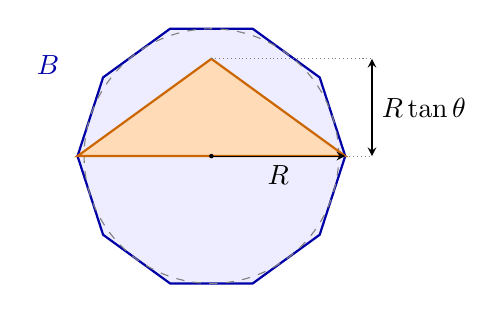
\begin{tikzpicture}[scale=1.7,>=stealth]
 \fill[blue!7] (0:1) \foreach \a in {36,72,...,324} {-- (\a:1)} -- cycle;
 \draw[blue!65!black,thick] (0:1) \foreach \a in {36,72,...,324} {-- (\a:1)} -- cycle;
 \draw[gray,dashed] (0,0) circle ({cos(18)});
 \filldraw[fill=orange!28,draw=orange!80!black,thick]
   (-1,0) -- (1,0) -- (0,{tan(36)}) -- cycle;
 \draw[->] (0,0) -- (1,0) node[midway,below] {$R$};
 \draw[gray,densely dotted] (0,{tan(36)}) -- (1.2,{tan(36)});
 \draw[gray,densely dotted] (1,0) -- (1.2,0);
 \draw[<->] (1.2,0) -- (1.2,{tan(36)})
    node[midway,right] {$R\tan\theta$};
 \fill (0,0) circle (.017);
 \node[blue!65!black] at (-1.22,.68) {$B$};
\end{tikzpicture}
\caption{A normal triangle translated into the reference decagon $B$.
Its longest side joins antipodal vertices, and its apex lies inside the
dashed incircle, of radius $R\cos(\theta/2)$. The other templates admit
the same placement in their prescribed orientations.}
\label{fig:pentagon-symmetric-calibration}
\end{figure}

Now $\lambda_B(K)B\subseteq K$. Monotonicity and homogeneity in the first
factor give
\[
 c(K\times_L Q)\ge\lambda_B(K)c(B\times_L Q)=\lambda_B(K),
\]
proving the capacity formula. The same containment yields
$\operatorname{area}(K)\ge\lambda_B(K)^2\operatorname{area}(B)$.
Since
\[
 \operatorname{area}(B)=5R^2\sin\theta,\qquad
 \operatorname{area}(Q)=\tfrac52\sin(2\theta),\qquad
 \frac1{2\operatorname{area}(B)\operatorname{area}(Q)}
 =\frac{10+6\sqrt5}{25},
\]
this proves the ratio bound. A proper inclusion between full-dimensional
convex bodies strictly increases area, so equality forces
$K=\lambda_B(K)B$ after translation. These partners also attain equality.
\end{proof}

The capacity formula can equivalently be expressed using the difference
body. Since $B=\tfrac12(Q-Q)^\circ$ and $K-K=2(K-z)$ for a symmetric
partner,
\[
 c(K\times_L Q)=W_Q(K),\qquad
 W_Q(K):=\max\{r\ge0:r(Q-Q)^\circ\subseteq K-K\}.
\]
For an arbitrary partner $K$, a segment translates into $K$ exactly when
its displacement lies in $K-K$. The same curve-cover argument gives
$c(K\times_L Q)\le W_Q(K)$.
Its central symmetrization $S=(K-K)/2$ satisfies $S-S=K-K$, so
\[
 W_Q(K)=c(S\times_L Q).
\]
Thus the width ceiling is precisely the capacity of the symmetrized
partner. The theorem shows that a partner violating the volume--capacity
inequality with this fixed pentagon must be asymmetric; equality with the
width ceiling for arbitrary asymmetric partners does not follow.
\FloatBarrier
